\documentclass[11pt,a4paper,oneside,openright,titlepage,
  headinclude,footinclude,BCOR5mm,
  numbers=noenddot,cleardoublepage=empty,
  tablecaptionabove, dottedtoc,
  bibliography=totoc]{scrreprt}
\usepackage{subfig}
\usepackage[
    eulerchapternumbers,
    subfig,
    beramono,
    eulermath,
    pdfspacing
  ]{classicthesis} 
\usepackage{arsclassica}
\usepackage{graphicx}
\usepackage[norsk,american]{babel}
\usepackage[utf8]{inputenc}
\usepackage[T1]{fontenc}
\usepackage{pdfpages}
\usepackage{titlesec}

\usepackage[numbers]{natbib}
\bibliographystyle{plainnat}

% *******************************************************
% DEFINE VARIABLES
% *******************************************************
\newcommand{\myName}{Raju Rimal*, Trygve Almøy \& Solve Sæbø}
\newcommand{\myTitle}{Exploration of Multi-Response Multivariate Methods}
\newcommand{\mySubTitle}{An application of simrel}
\newcommand{\myLocation}{\spacedlowsmallcaps{Ås, Norway}}
\newcommand{\myGroup}{BIAS @ KBM, NMBU}
\newcommand{\myUrl}{\url{https://www.mathatistics.com/}}
\newcommand{\myTime}{2019, July}
\newcommand{\docsite}{\url{https://therimalaya.github.com/thesis}}
\newcommand{\email}{\mail{raju.rimal@nmbu.no}}

% *******************************************************
% CUSTOMIZATIONS
% *******************************************************
\newcommand{\mail}[1]{\href{mailto:#1}{\texttt{#1}}}
\titleformat{\part}[display]
  {\normalfont\centering\large}%
  {\thispagestyle{empty}\partname~\MakeTextUppercase{\thepart}}{1em}%
  {\color{Maroon}\spacedallcaps}

\begin{document}
\pagenumbering{Roman}
\pagestyle{plain}
% *******************************************************
% Title Front
% *******************************************************
\begin{titlepage}
  \pdfbookmark{Titlepage}{Titlepage}
  \null\vfill
  \begin{center}
    \large \sffamily
    \bigskip
    {\Large\spacedlowsmallcaps{\myName}} \\
    \bigskip
    {\huge\spacedlowsmallcaps{\myTitle} \\}
    \bigskip
    \vspace{9cm}
    \begin{tabular} {cc}
      \parbox{0.3\textwidth}{
\includegraphics[width=3.5cm]{Logo}}
      & \parbox{0.7\textwidth}{{\Large\spacedlowsmallcaps{\mySubTitle}} \\ 
      {\normalsize
      \myGroup \\
      \myUrl \\
      \myTime}}
    \end{tabular}
  \end{center}
  \vfill
\end{titlepage}

% *******************************************************
% Title Back
% *******************************************************
\thispagestyle{empty}
\hfill \vfill
\noindent\myName:
\textit{\myTitle,} \mySubTitle,
\textcopyright\ \myTime.
\medskip
\noindent{\spacedlowsmallcaps{Website}}: \\
\docsite

\medskip
\noindent{\spacedlowsmallcaps{E-mail}}: \\
\email

\vspace{1cm}
\hrule
\bigskip

\noindent The titlepage reproduces an engraving of Maurits Cornelis Escher, titled \emph{Plane Filling with Birds} (the picture is obtained from \url{http://www.mcescher.com/}).

\pagestyle{scrheadings} 
\clearpage

% *******************************************************
% ABSTRACT
% *******************************************************
\pdfbookmark{Abstract}{Abstract}
\begingroup
\let\clearpage\relax
\let\cleardoublepage\relax
\let\cleardoublepage\relax

\addchap{Abstract}
This section belongs to absctract. Write awesome abstract.
\vfill

% *******************************************************
% SUMMARY
% *******************************************************
\clearpage
\pdfbookmark[1]{Sommario}{Sommario}
\addchap{Summary}
This is summary section of the thesis.
\endgroup
\vfill

% *******************************************************
% ACKNOWLEDGMENT
% *******************************************************
\pdfbookmark{Acknowledgements}{Acknowledgements}

\begingroup
\let\clearpage\relax
\let\cleardoublepage\relax
\let\cleardoublepage\relax

\addchap{Acknowledgements}

I wish first of all to thank the members of the Staff of the Italian \TeX\{\} and \LaTeX\{\} User Group, in particular Prof.\textasciitilde Enrico Gregorio, for their invaluable aid during the writing of this work, the detailed explanations, the patience and the precision in the suggestions, the supplied solutions, the competence and the kindness. Thanks also to all the people who have discussed with me on the forum of the Group, prodigal of precious observations and good advices.

Finally, thanks to Andr'e Miede, for his wonderful ClassicThesis style, and to Daniel Gottschlag, who gave to me the hint for this original reworking.

\endgroup

% *******************************************************
% Contents
% *******************************************************
\clearpage
\phantomsection
\pdfbookmark{\contentsname}{tableofcontents}
\setcounter{tocdepth}{2}
\begingroup 
  \let\clearpage\relax
  \let\cleardoublepage\relax
  \tableofcontents
\endgroup
\markboth{\spacedlowsmallcaps{\contentsname}}
{\spacedlowsmallcaps{\contentsname}} 

\begingroup 
  \let\clearpage\relax
  \let\cleardoublepage\relax
\endgroup

\cleardoublepage
% *******************************************************
% BODY START
% *******************************************************
\pagenumbering{arabic}


\hypertarget{introduction}{%
\chapter{Introduction}\label{introduction}}

Citing \citet{rimal2019pred} in this text.

\hypertarget{methods}{%
\chapter{Methods}\label{methods}}

This is the introduction section. It contains background subsection

\hypertarget{background}{%
\section{Background}\label{background}}

Here I will reference to \citep{naes2013multi} I hope this will render properly.

% *******************************************************
% BIBLIOGRAPHY START
% *******************************************************
 % biblio-title
 % beamer
  \bibliography{References.bib}
 % beamer
 % bibliography
 % natbib


 % biblatex

\nocite{*}

% *******************************************************
% PAPER START
% *******************************************************
\appendix
\part*{Research Papers}
\par\chapter{A tool for simulating multi-response linear model data}

\includepdf[pages=-]{papers/001.pdf}
\par\chapter{Model and estimators for partial least squares regression}

\includepdf[pages=-]{papers/002.pdf}
\par\chapter{Comparison of Multi-response Prediction Methods}
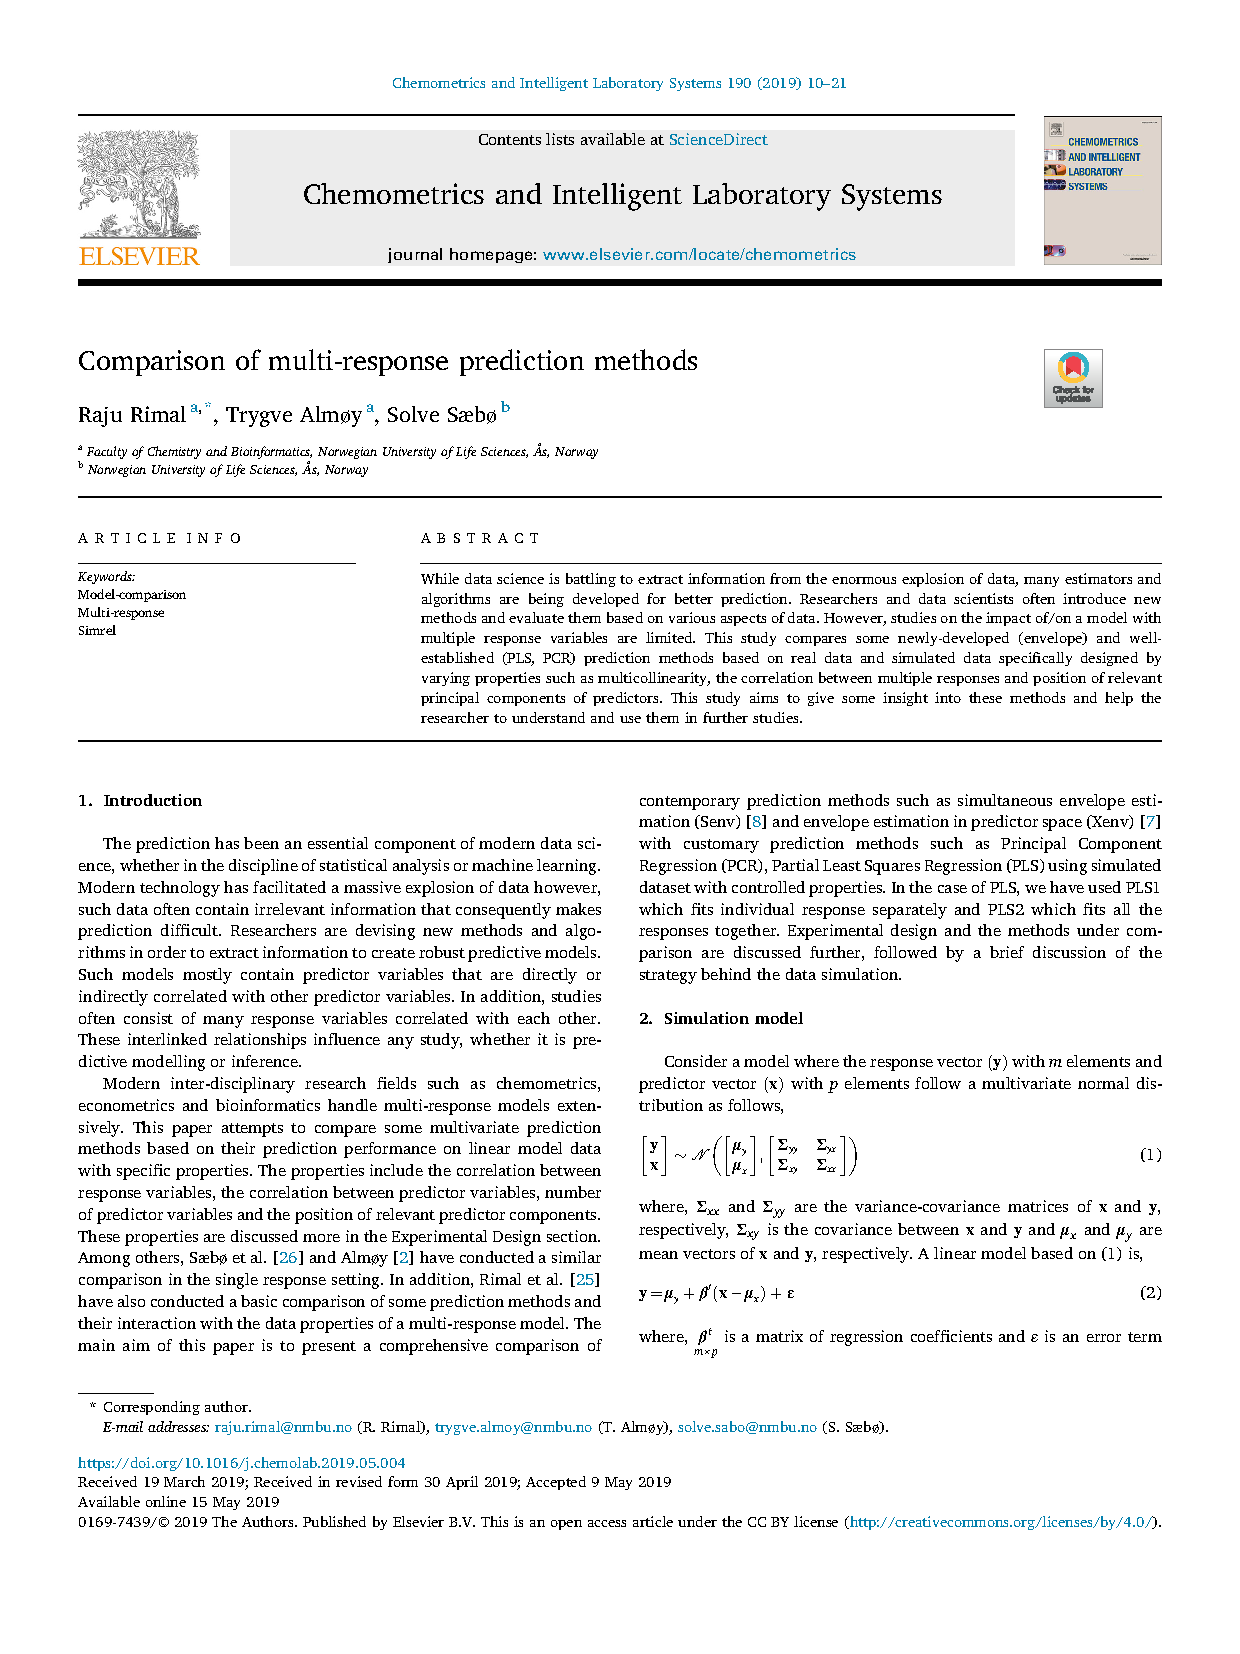
\includepdf[pages=-]{papers/003.pdf}
% \par\chapter{Paper1: A tool for simulating multi-response linear model data}
% 
\includepdf[pages=-]{papers/001.pdf}
% \par\chapter{Paper2:  Model and estimators for partial least squares regression}
% 
\includepdf[pages=-]{papers/002.pdf}
% \par\chapter{Paper3: Comparison of Multi-response Prediction Methods}
% 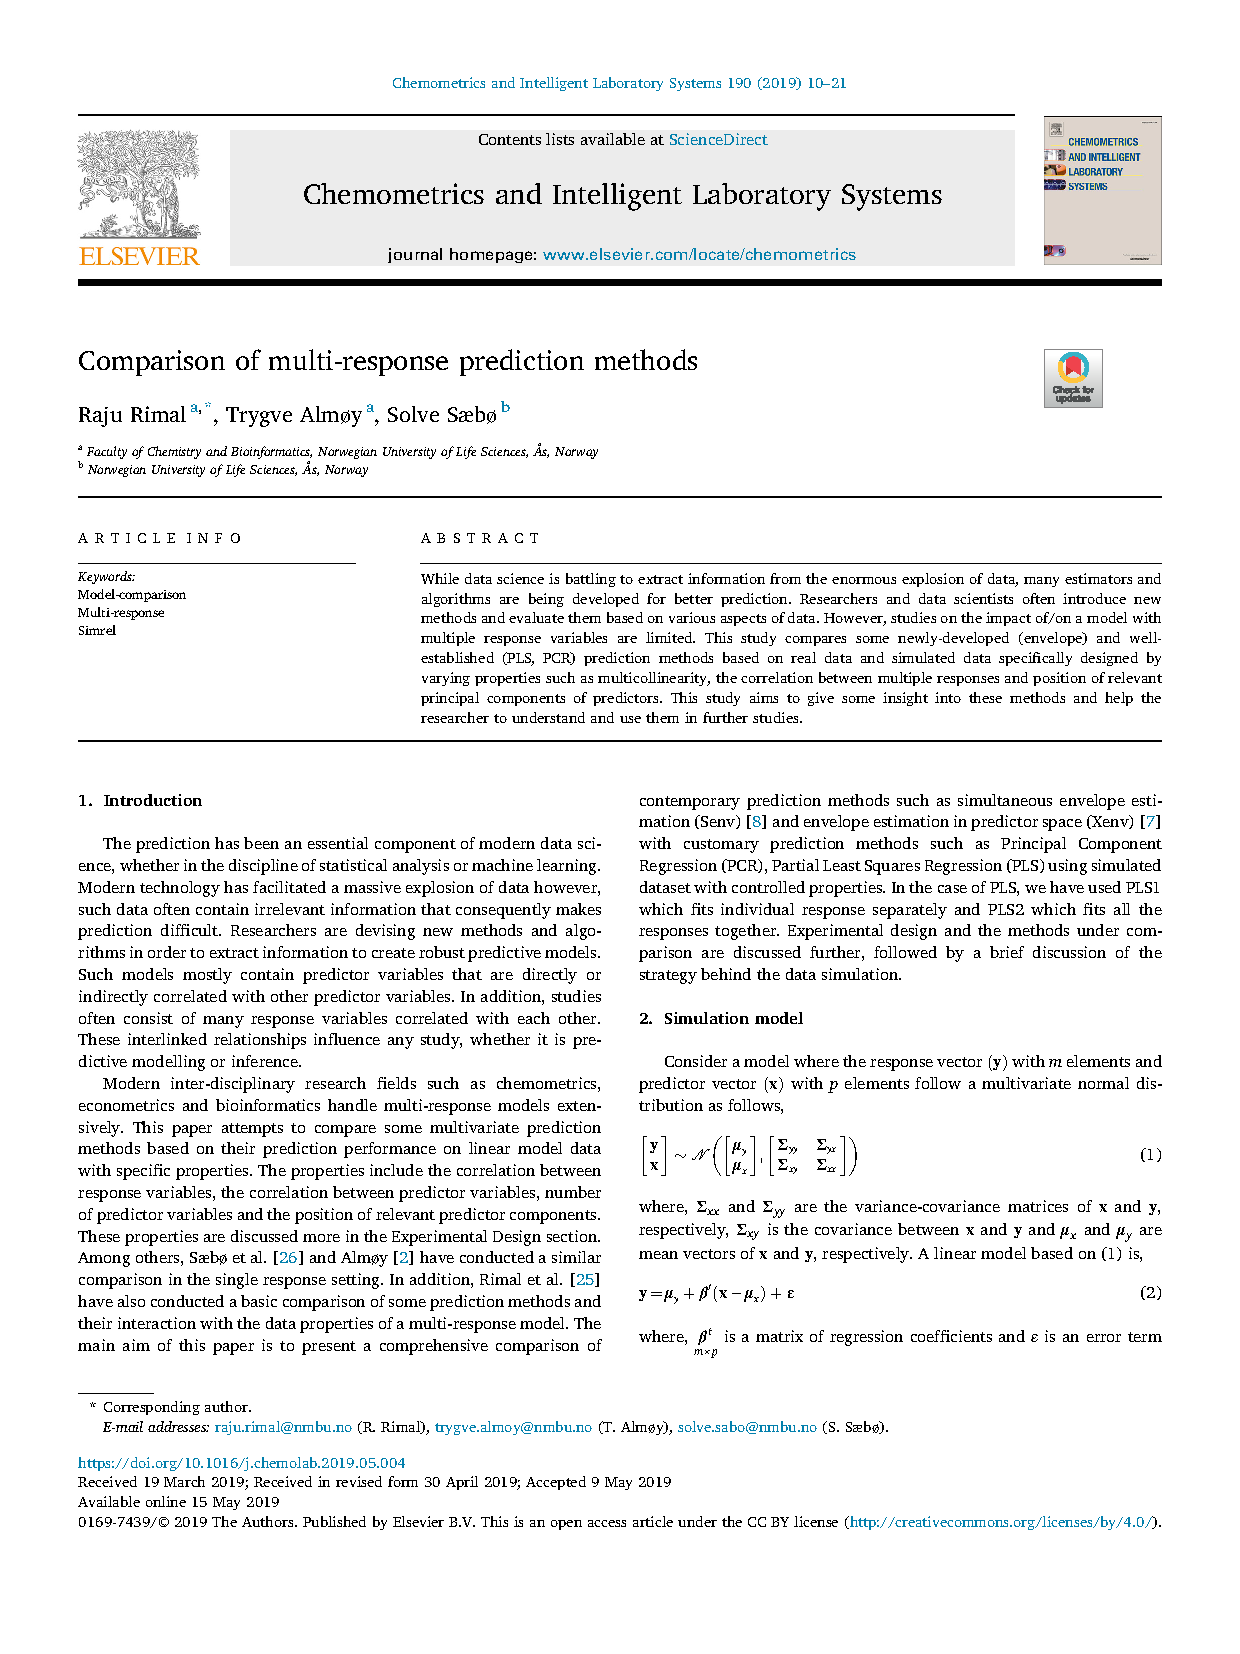
\includepdf[pages=-]{papers/003.pdf}

% *******************************************************
% ANYTHING EXTRA
% *******************************************************

\end{document}

%%% Local Variables:
%%% mode: latex
%%% TeX-master: t
%%% End:
